\chapter{Appendix 2}
\section{2D topology optimization examples}
\label{examples_to2D}
\subsubsection{MBB optimization}
The MBB beam optimization problem is a very common test case in topology optimization. It is often modeled considering the symmetry of geometry, loads and boundary conditions c.f. figure \ref{fig.2.11}.
\begin{figure}[ht]
\centering
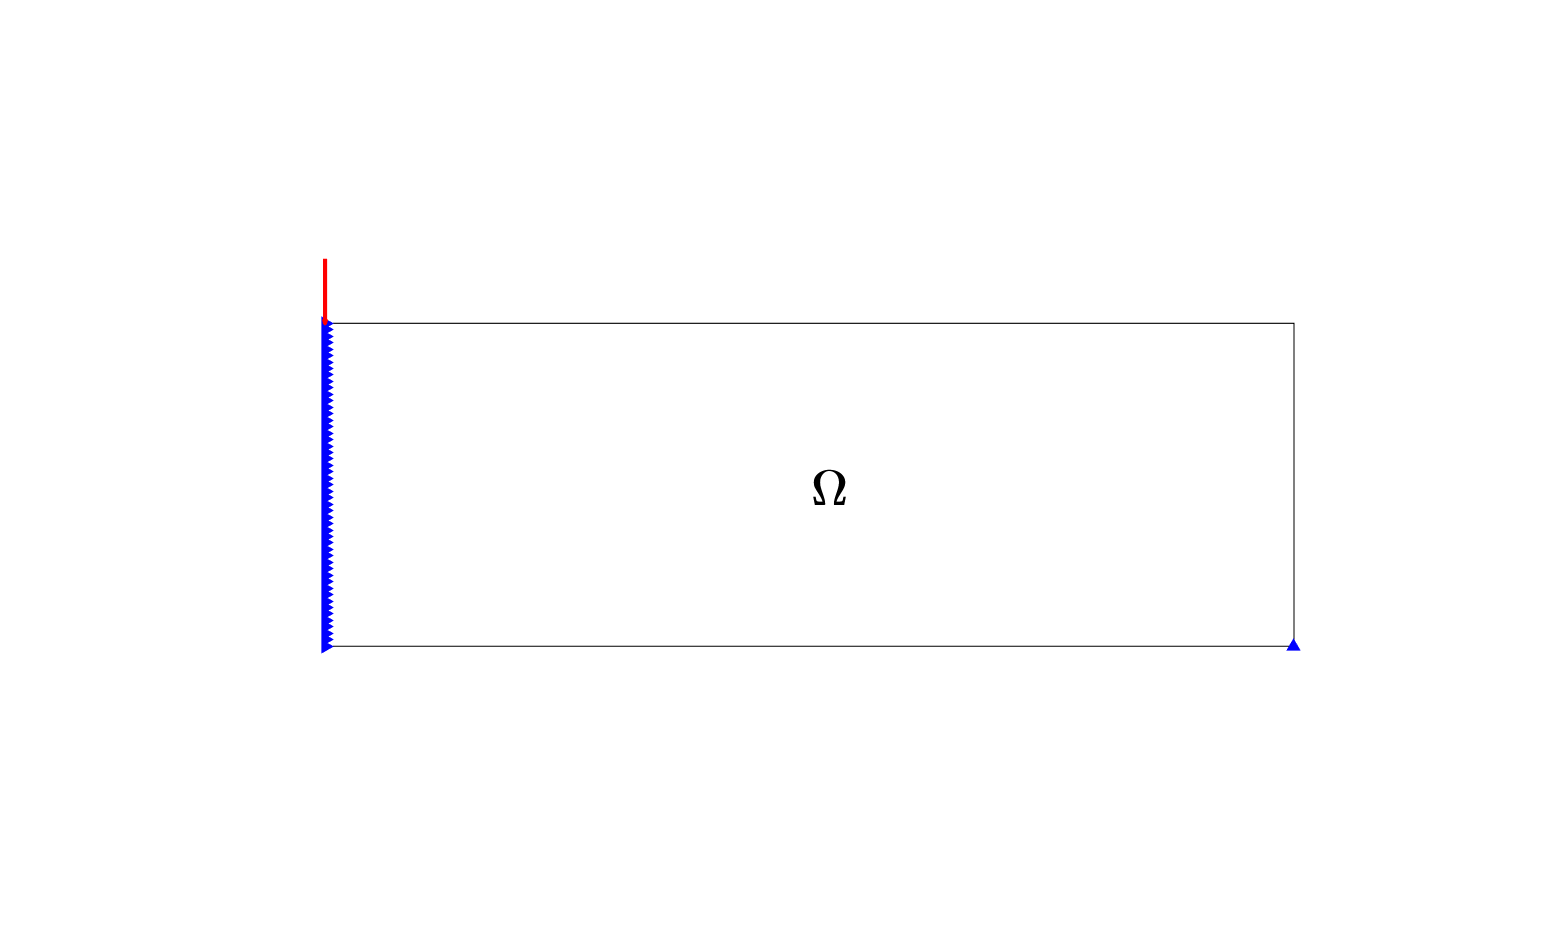
\includegraphics[width=\textwidth]{images/Ch2/design_problem}
\caption{Geometry, Load and boundary conditions of the MBB topology optimization problem. Blue triangles are oriented as the fixed DOFs. The red arrow represents the applied load and point through the position of node were the load is applied.}
\label{fig.2.11}
\end{figure}
We adopted 2 meshes to solve this problem one of $150\times50$ and the other of $300\times100$. To have a mesh independent solution the initial radius was set in the first case to 6 and in the second to 12. The results and the convergence history of each optimization is shown in figure \ref{fig.2.12}. 
\begin{figure}[hbt!]
  \centering
       \subfloat[ \label{fig.2.12c}]{%
                       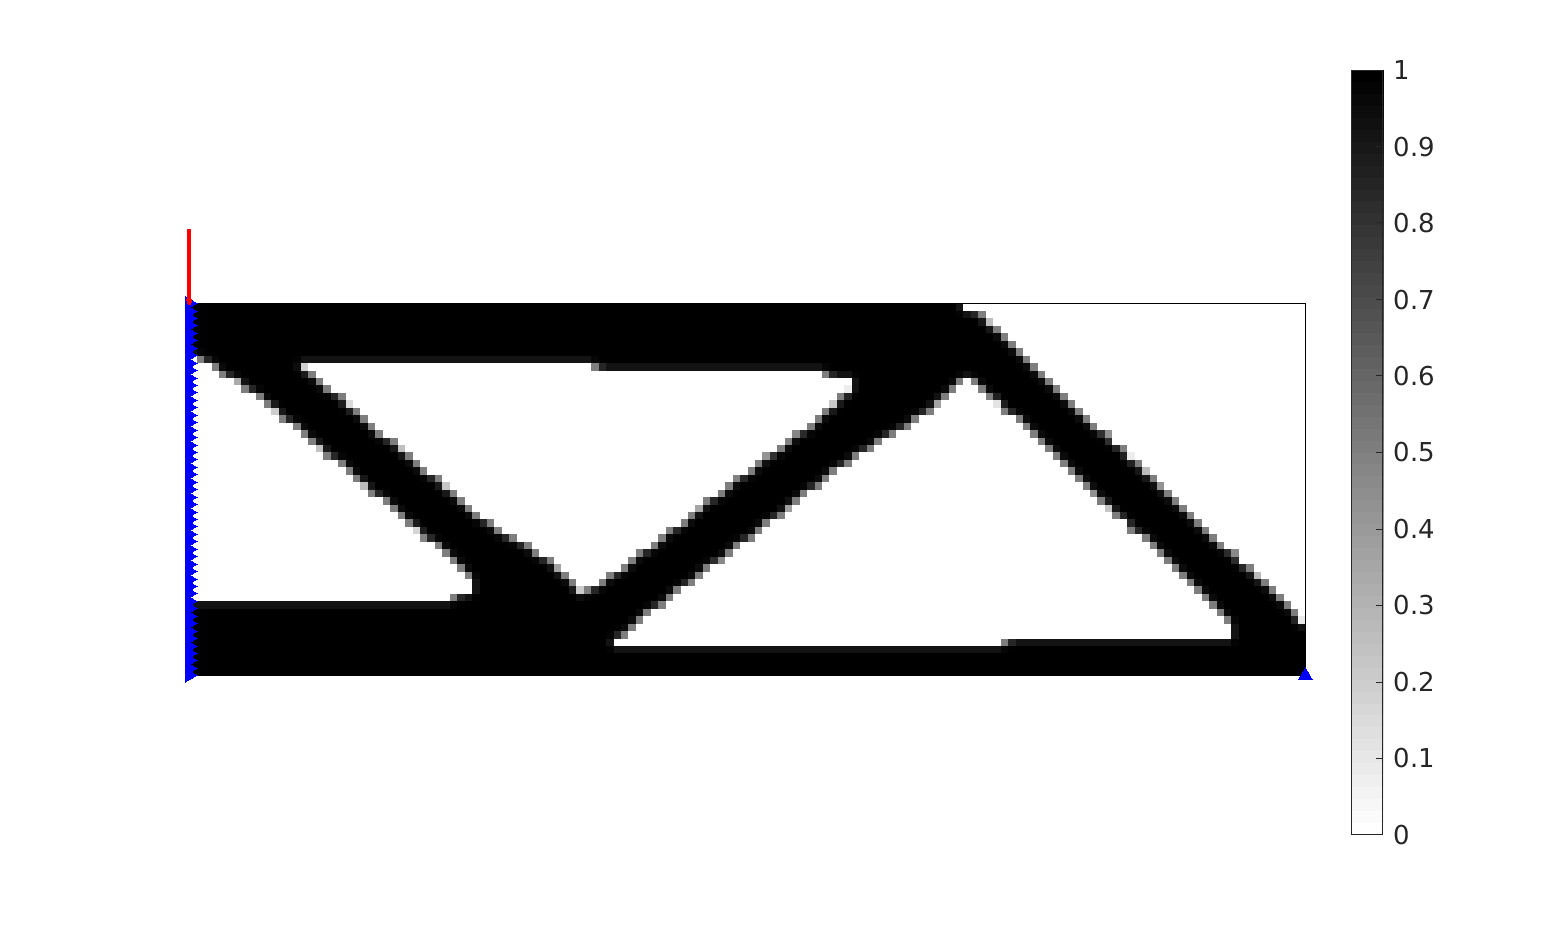
\includegraphics[width=0.5\textwidth]{images/Ch2/MBBnelx_150nely_50_R_6_volfrac_40_ft_3density}
                     }
              \subfloat[  \label{fig.2.12d}]{%
                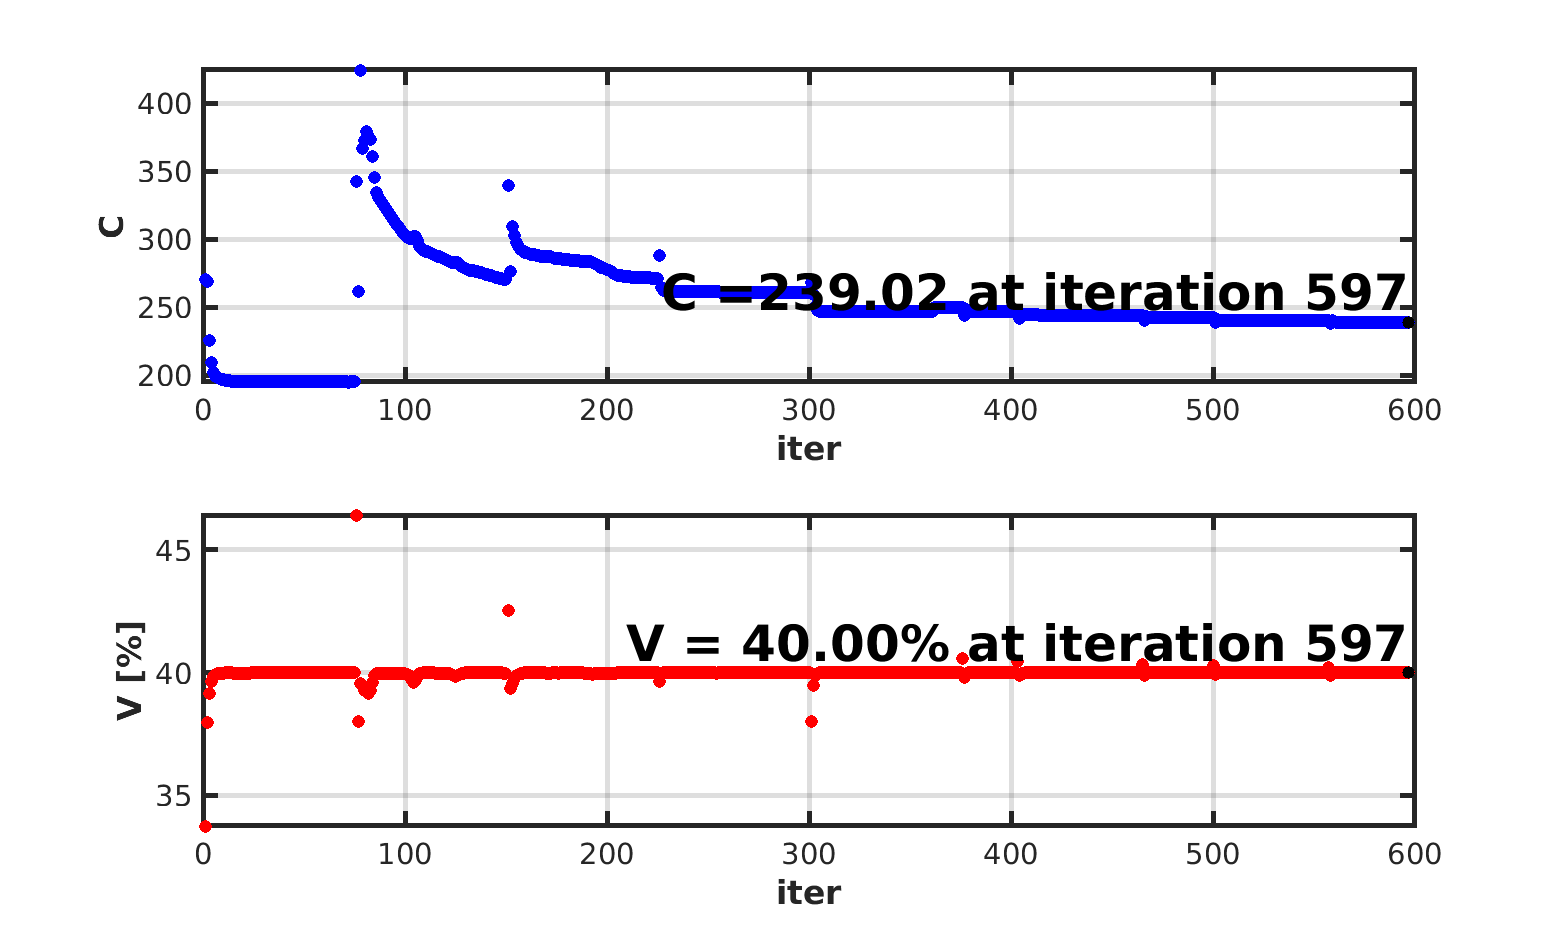
\includegraphics[width=0.5\textwidth]{images/Ch2/MBBnelx_150nely_50_R_6_volfrac_40_ft_3convergence}
              }
              \\
               \subfloat[ \label{fig.2.12a}]{%
                              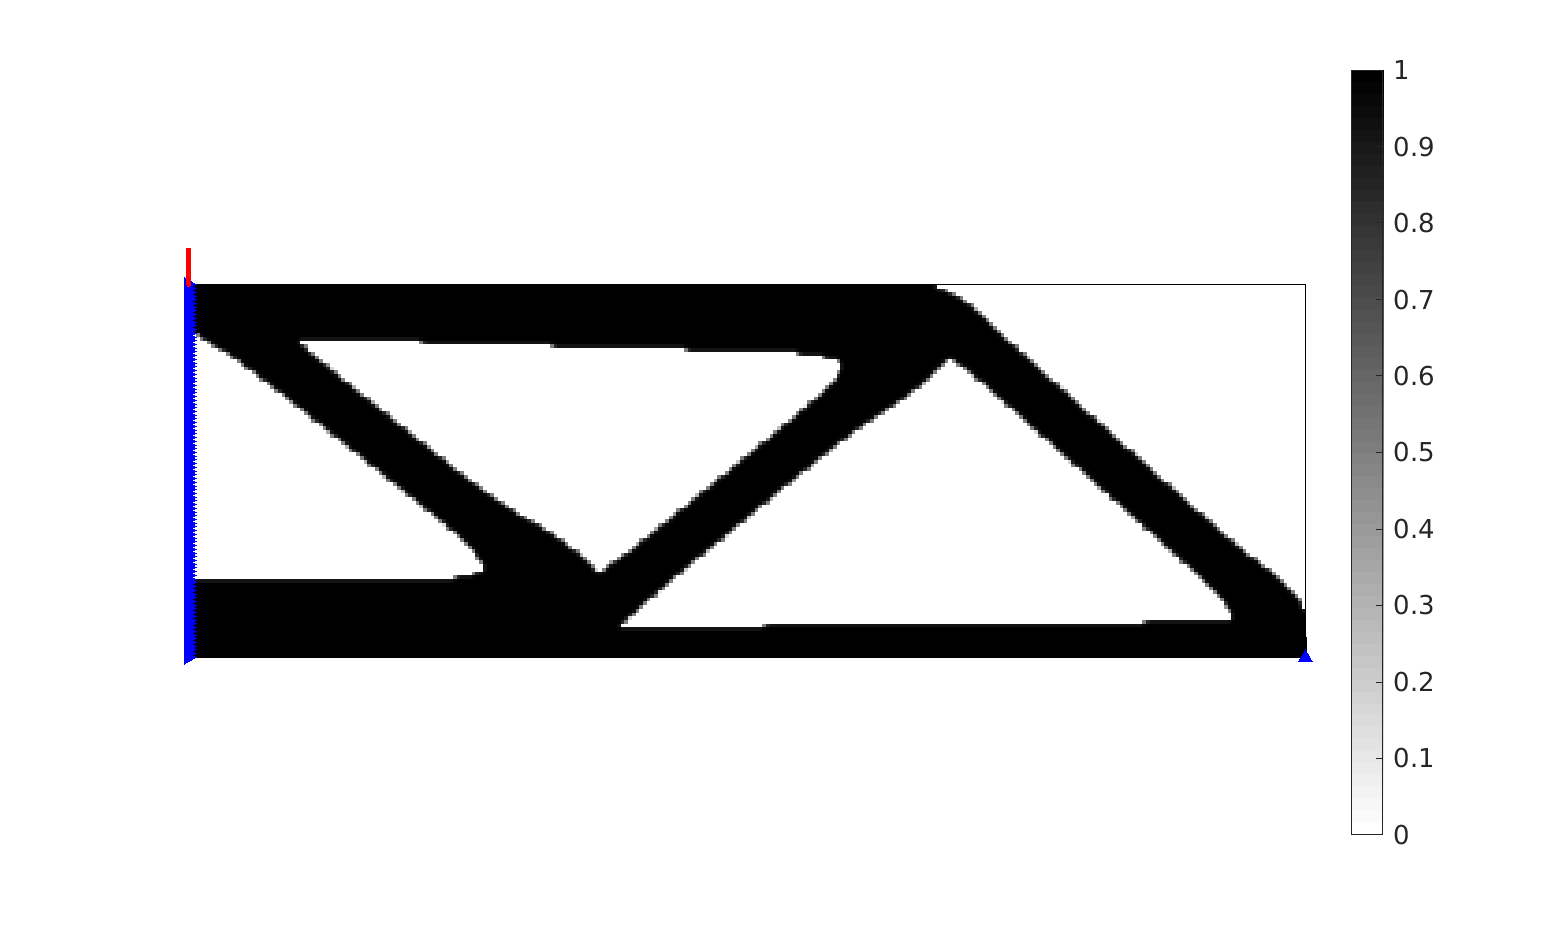
\includegraphics[width=0.5\textwidth]{images/Ch2/MBBnelx_300nely_100_R_12_volfrac_40_ft_3density}
                            }
                     \subfloat[  \label{fig.2.12b}]{%
                       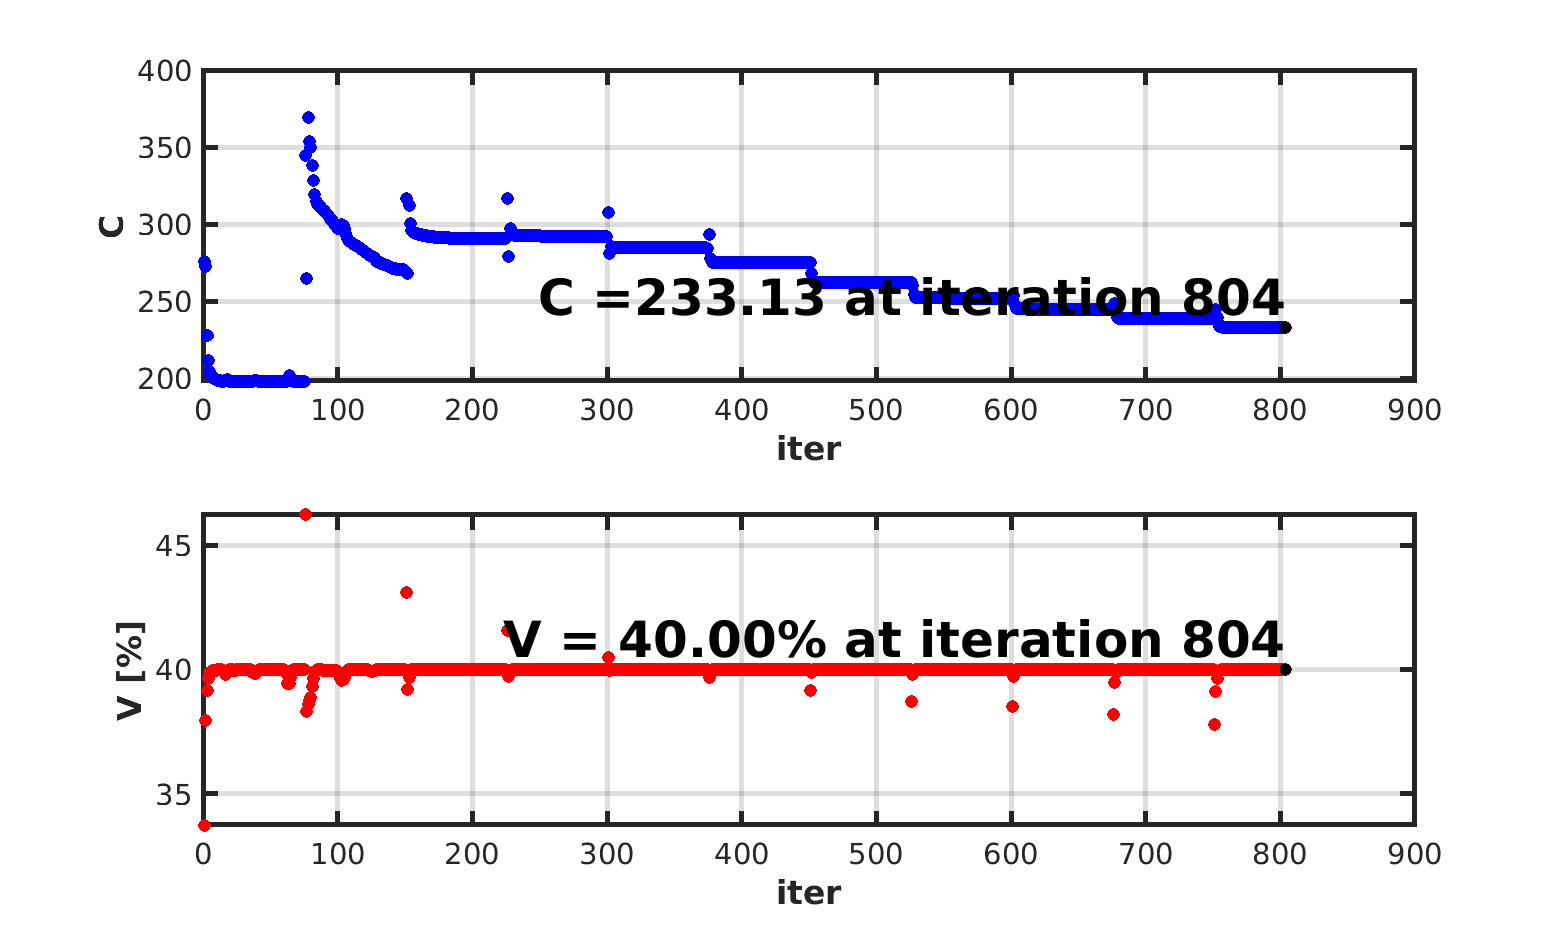
\includegraphics[width=0.5\textwidth]{images/Ch2/MBBnelx_300nely_100_R_12_volfrac_40_ft_3convergence}
                     }
       \caption{MBB topology optimization results. (a)-(b) $\VectorVar{x_{Phys}}$ distribution and responses convergence for the $150\times 50$ discretization.(c)-(d) $\VectorVar{x_{Phys}}$ distribution and responses convergence for the $300\times 100$ discretization }
       \label{fig.2.12}
     \end{figure}
     One can observe from figure \ref{fig.2.12a} and \ref{fig.2.12c} that the solution found is independent from the mesh found. The choice of both filer radius and continuation strategy helps in the determination of this design. Moreover the solution have small transitions region on the boundary of the solid. This is thanks to the Heaviside filter and the continuation strategy adopted for $\beta$. Thanks to that, exploiting this results is easier. In fact using a threshold it is possible to convert these solutions to a black and white (0-1) design that will be close enough to the actual optimization solution.  On figures \ref{fig.2.12b} and \ref{fig.2.12d} one can observe a quite long converge history for both meshes. This is due to the continuation strategy adopted here. Moving forward, this design is an actual local minimum that respect all constraints as it can be observed from both figures \ref{fig.2.12b} and \ref{fig.2.12d}. In fact even if the convergence criterion on design vector change was not reached, in the final iterations the variations of both objective function and volume constraint are very small. The FEM is still valid on the optimum even if $150\times50$ is slightly softer. This can be an effect of differences in the solutions.
      The small displacement hypothesis cannot be verified here since all measures considered for this test case are dimensionless. Finally being the final application and the technology adopted for the manufacturing not specified, we cannot make any conclusions about the acceptability of this design candidate or of the model validity.
     \clearpage
\subsubsection{Short cantilever beam optimization}
This second use-case is also very well known and studied in the literature. A domain design is clamped on the left side and excited on the right side c.f. figure \ref{fig.2.13}.
\begin{figure}[ht]
\centering
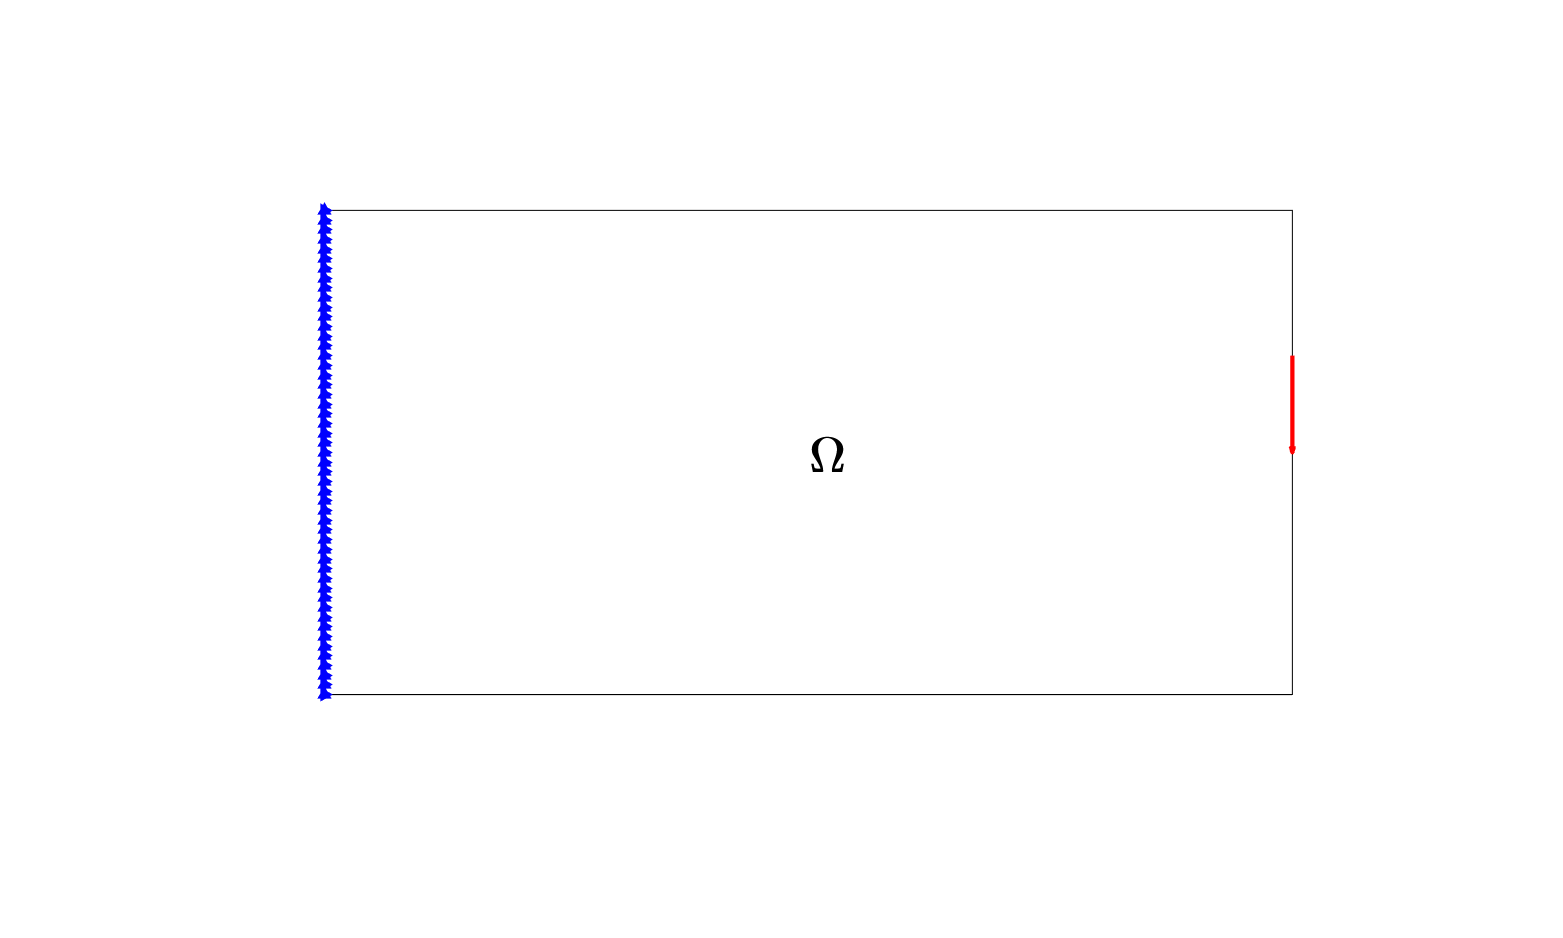
\includegraphics[width=\textwidth]{images/Ch2/design_problem2}
\caption{Geometry, Load and boundary conditions of the short cantilever topology optimization problem. Blue triangles are oriented as the fixed DOFs. The red arrow represents the applied load and point through the position of node were the load is applied.}
\label{fig.2.13}
\end{figure}
We adopted 2 meshes to solve this problem one of $100\times50$ and the other of $200\times100$. To have a mesh independent solution the initial radius was set in the first case to 6 and in the second to 8. The results and the convergence history of each optimization is shown in figure \ref{fig.2.14}. 
\begin{figure}[hbt!]
  \centering
       \subfloat[ \label{fig.2.14a}]{%
                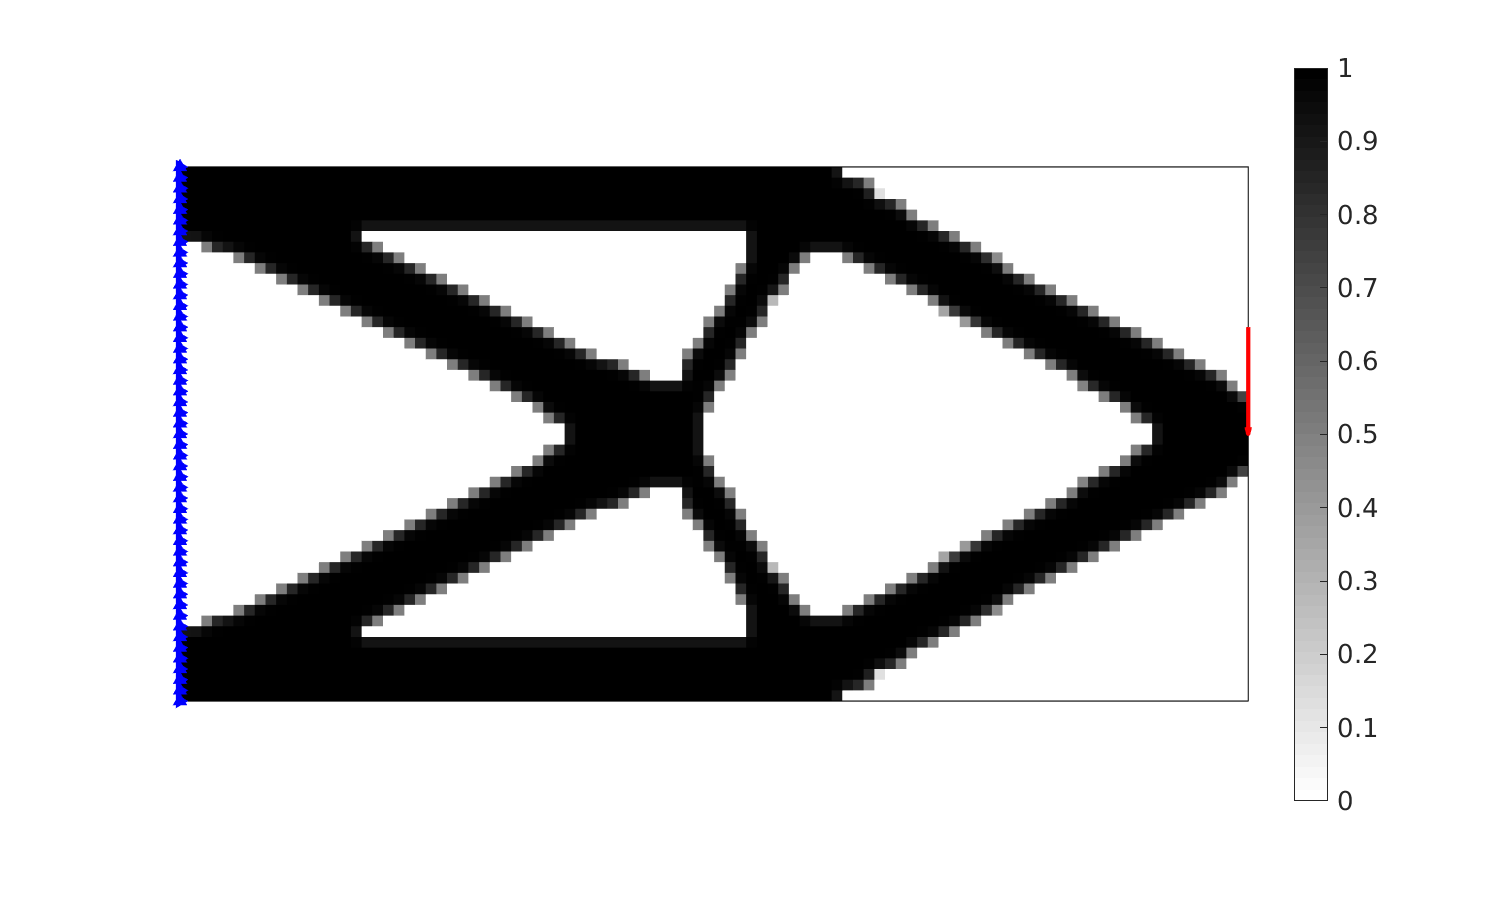
\includegraphics[width=0.5\textwidth]{images/Ch2/Short_Cantilevernelx_100nely_50_R_6_volfrac_40_ft_3density}
              }
       \subfloat[  \label{fig.2.14b}]{%
         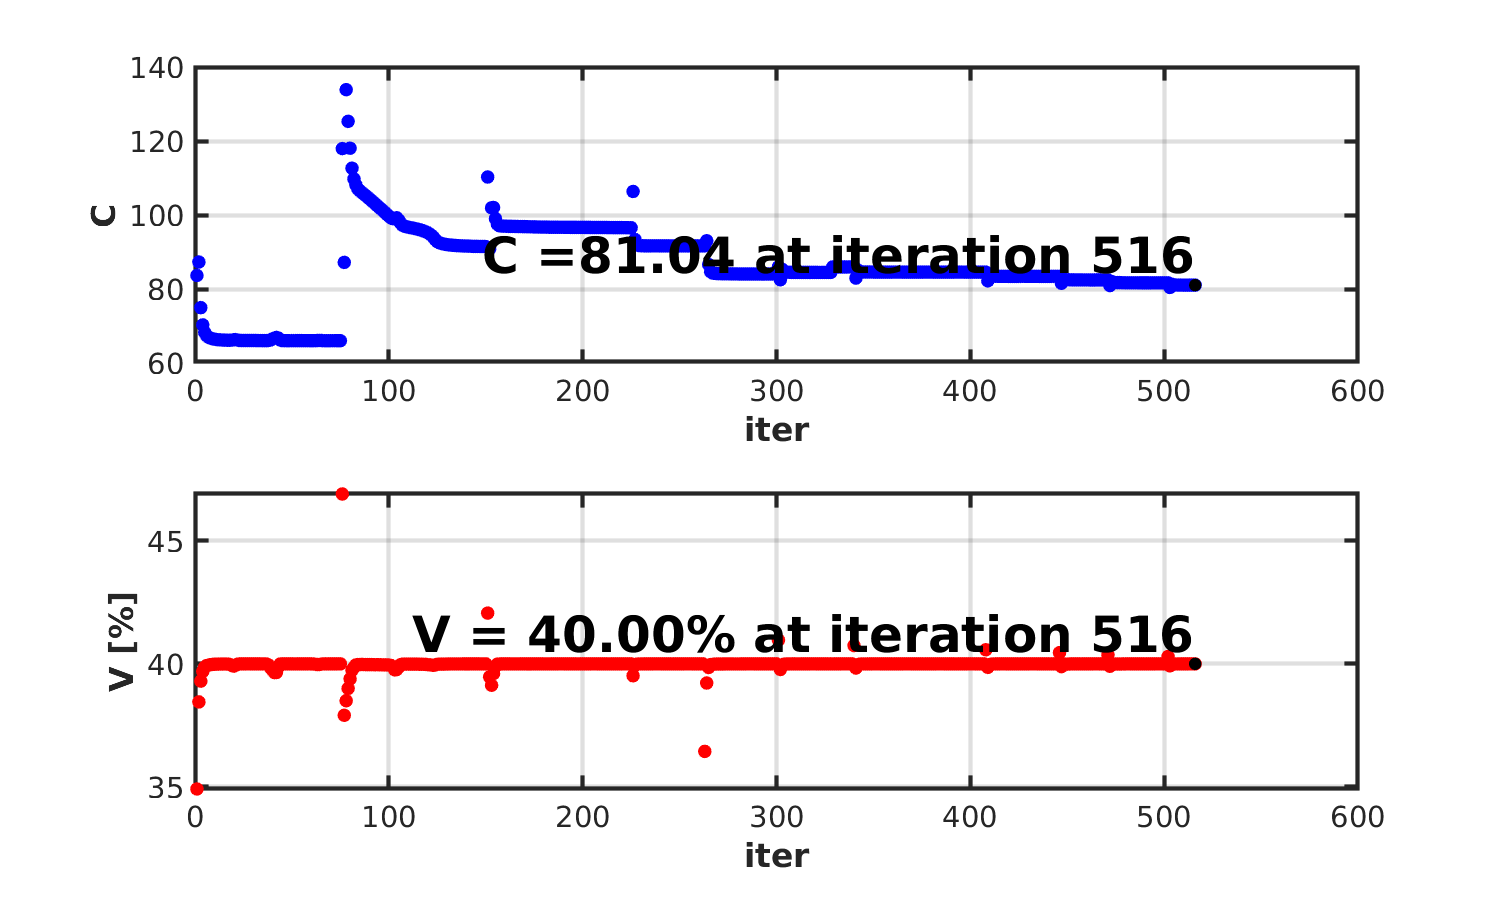
\includegraphics[width=0.5\textwidth]{images/Ch2/Short_Cantilevernelx_100nely_50_R_6_volfrac_40_ft_3convergence}
       }
       \\
       \subfloat[ \label{fig.2.14c}]{%
                       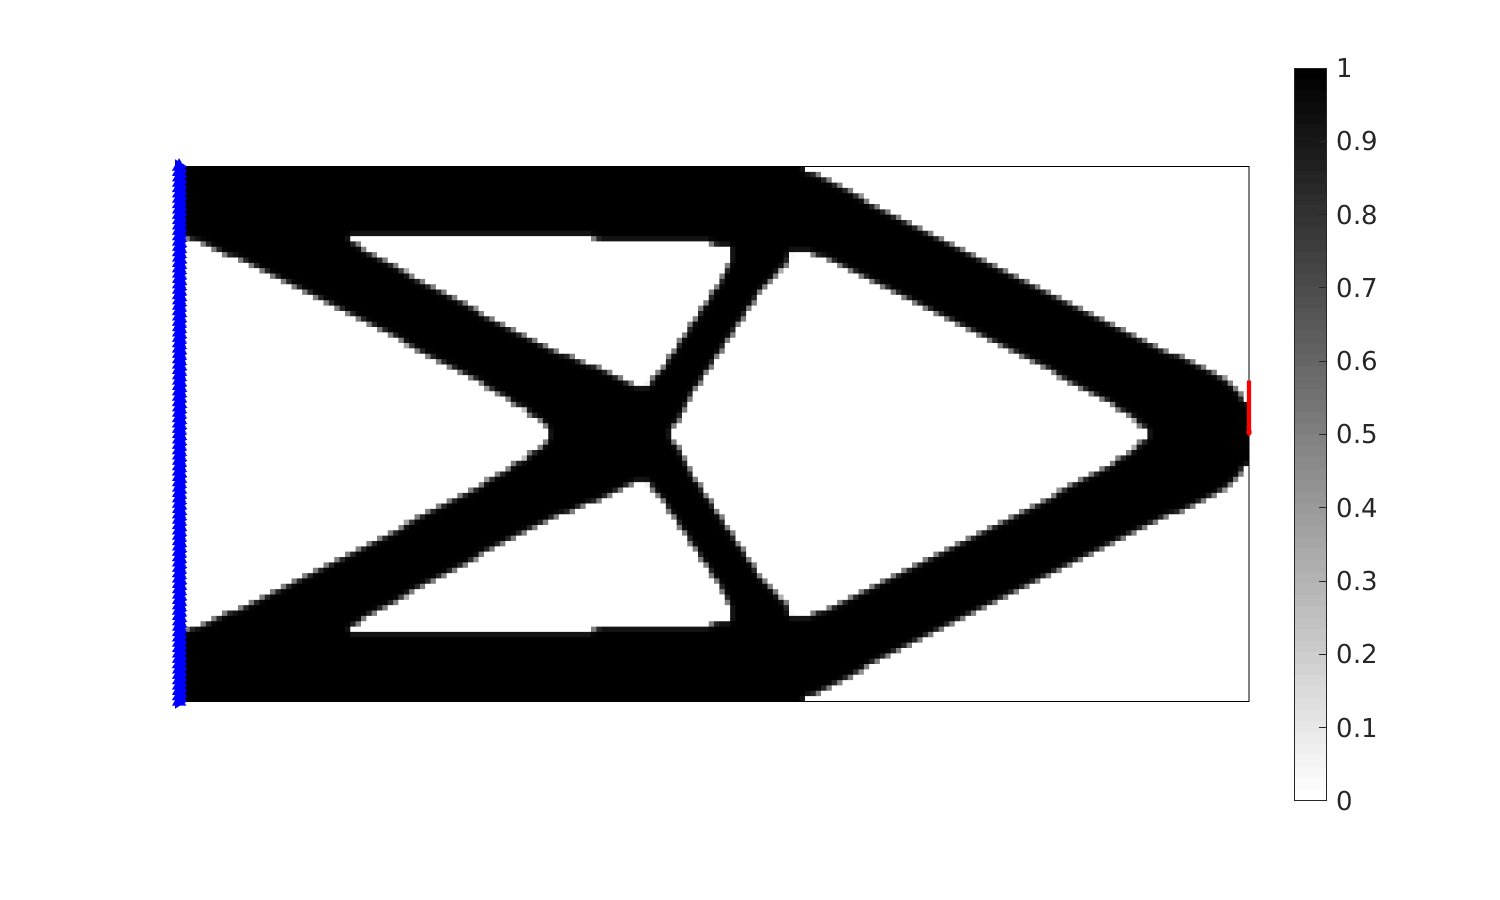
\includegraphics[width=0.5\textwidth]{images/Ch2/Short_Cantilevernelx_200nely_100_R_8_volfrac_40_ft_3density}
                     }
              \subfloat[  \label{fig.2.14d}]{%
                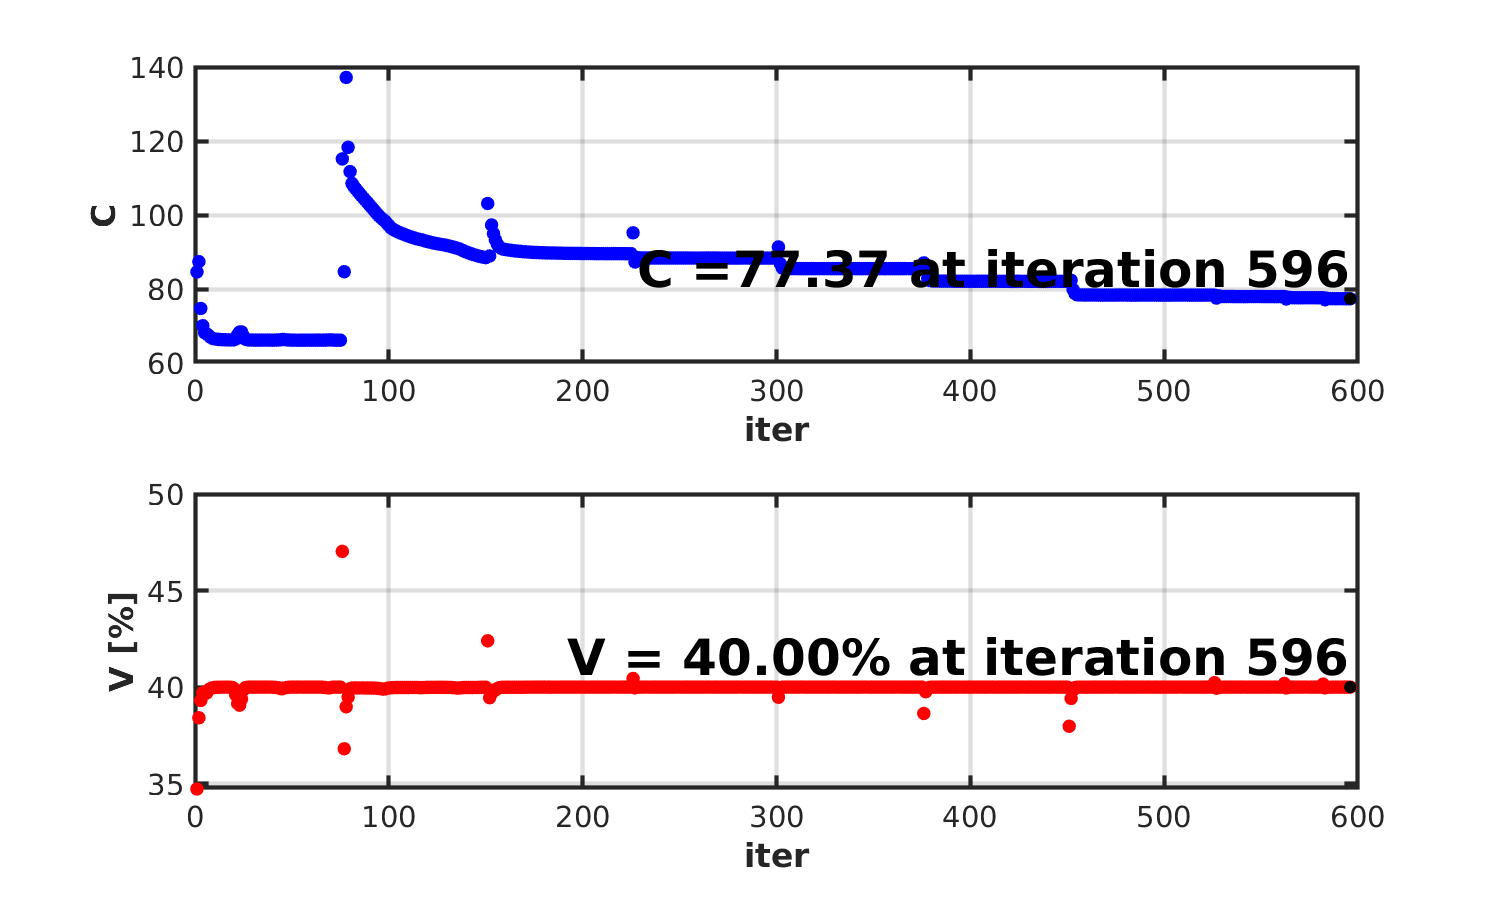
\includegraphics[width=0.5\textwidth]{images/Ch2/Short_Cantilevernelx_200nely_100_R_8_volfrac_40_ft_3convergence}
              }
       \caption{Short cantilever topology optimization results. (a)-(b) $\VectorVar{x_{Phys}}$ distribution and responses convergence for the $100\times 50$ discretization.(c)-(d) $\VectorVar{x_{Phys}}$ distribution and responses convergence for the $200\times 100$ discretization }
       \label{fig.2.14}
     \end{figure}
     The solutions obtained for different discretizations are also this time very similar c.f. figures \ref{fig.2.14a} and \ref{fig.2.14c}. Nearly black and white solutions are determined. The convergence figures history \ref{fig.2.14b} and \ref{fig.2.14d}, tell us that both optimization were converged this time respecting the design variable change criterion. Both solution found are symmetric with respect to the middle axis. Also this time one can identify 8 thin members composing the solution. The design found by the finer discretization is slightly stiffer then the one fond by the coarser mesh. Also this time one can find an explanation either in small discrepancies between solutions. Again any conclusions can be outlined on the model validity and the design acceptability on the base of the data of the problem in hand.
     \clearpage
\section{KS function properties}
\label{Appendix1}
In the following subsection we review essential properties of the Kreisselmeier-Steinhauser (KS) functions used for the stress constraints.
Given that $P\left(\bar{g}_i-\bar{g}_{max}\right)\leq 0$, $\forall i$ , $e^{P\left(\bar{g}_i-\bar{g}_{max}\right)}\leq 1$, $\forall i$ and $\frac{1}{P}\ln\left(\sum_{i=1}^{N_G}e^{P\left(\bar{g}_i-\bar{g}_{max}\right)}\right)-\frac{\ln\left(N_G\right)}{P}\leq 0$ so that one can conclude $G^{l}_{KS}\leq \bar{g}_{max}$ and knowing that  $\sum_{i=1}^{N_G}e^{P\left(\bar{g}_i-\bar{g}_{max}\right)}>1$ implies $\frac{1}{P}\ln\left(\sum_{i=1}^{N_G}e^{P\left(\bar{g}_i-\bar{g}_{max}\right)}\right)>0$ so that:
\begin{equation}
\label{eq.NGP}
\bar{g}_{max}-G^{l}_{KS}=\frac{\ln\left(N_G\right)}{P}-\frac{1}{P}\ln\left(\sum_{i=1}^{N_G}e^{P\left(\bar{g}_i-\bar{g}_{max}\right)}\right)< \frac{\ln\left(N_G\right)}{P}
\end{equation}
As a remarkable results we have:
 \begin{equation}
 G^{l}_{KS}\leq\bar{g}_{max}<G^{l}_{KS}+\frac{\ln\left(N_G\right)}{P}=G_{KS}
 \end{equation}
 Where $G_{KS}$ is the Kreisselmeier-Steinhauser function.
Equivalently:
  \begin{equation}
  \label{ee20}
  0\leq\bar{g}_{max}-G^{l}_{KS}<\frac{\ln\left(N_G\right)}{P}
  \end{equation} 
Finally $\lim\limits_{P\rightarrow \infty}\frac{\ln\left(N_G\right)}{P}=0$
that for eq. \ref{ee20} implies:
\begin{equation}
\lim\limits_{P\rightarrow \infty}G^{l}_{KS}=\bar{g}_{max}
\end{equation}
One can also limit the range of variation of $\bar{g}_{max}$ using an allowable tolerance: 
\begin{equation}
\left|G^{l}_{KS}-\bar{g}_{max}\right|<\epsilon 
\end{equation}
According to eq. \eqref{eq.NGP} one can chose a value of P of
\begin{equation}
  P>\frac{\ln\left(N_G\right)}{\epsilon} 
\end{equation}
One must also keep in mind that for greater value of $P$, the $G_{KS}^l$ can have very non-linear behavior. This has some negative consequences on gradient based optimization solver. An opposite strategy to deal with stress non linearity was explored in Lian et al. \cite{lian2017combined}. In this paper they proposed to increase the number of Gauss Points $N_G$. According to equation \eqref{eq.NGP} this strategy increase the distance from the true maximum function hence reducing the stress aggregation function non linearities. When using lower bound KS function and p-mean this difference is inconvenient because the final maximum stress will be greater than the one  corresponding to KS aggregation, needing compensation on the stress limit (as suggested in this paper). On the other hand using KS function or p-norm the design is always slightly oversized, so that increasing the aggregation constant could still be beneficial to the final mass of the solution. A less elegant, but still effective way of accounting for this gap is to change allowable stress during iterations in the way proposed in Le et al. \cite{le2010stress}.   
\section{TSFC constraint parametric study}
\label{TSFCpareto}
In this section we propose to study the impact of the TSFC variation constraint on the solution of problem in Eq. \ref{topoeq3}. This is interesting to extract some conclusions on:
\begin{itemize}
\item The quantification of the possible impact of pylon and engine mount design on the TSFC variation.
\item The quantification of the mass investments required to achieve a given tip clearance control improvement.
\item The detection of key design features that can help controlling tip clearance.
\end{itemize} 
Solution A, B, C, D represented in figures \ref{fig.B22},\ref{fig.B23},\ref{fig.B24},\ref{fig.B25} are obtained with $T_0=0.16,0.17,0.18,1$ respectively. The corresponding value of aggregated TSFC variation and aggregated Compliance is shown figure \ref{fig.B21}. 
One can then outline the following conclusions:
\begin{itemize}
\item When lower value of TSFC variation are enforced, the final volume fraction is increased, that shows that these two responses are antagonistic.
\item The solution D has a final aggregated TSFC variation of 0.183 smaller then the bound of 1. This means that TSFC constraint is not active for this optimization and that the only stress constraint was activated.
\item Solution C and B improve both compliance and TSFC variation compared to solution D. On the other hand solution A is heavier and softer than the other solutions.
\item Solution A (c.f. figure \ref{fig.B22} ) is very different from the other solutions (c.f. figures \ref{fig.B23},\ref{fig.B24} and \ref{fig.B25}). The frontal part is stiffened but has a much softer rear part with respect to lateral loads. 
\item The frontal part is stiffened passing from solution D to solution A, in particular connection between core casing and Outlet Guide Vain basis is reinforced. The seems to be a key connection for engine deformation control.
\end{itemize} 
\begin{figure}[hbt!]
  \centering
       \subfloat[ \label{fig.B21a}]{%
                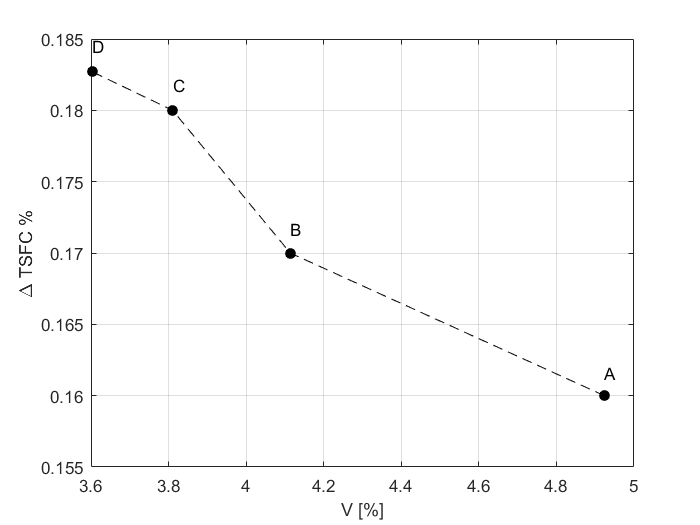
\includegraphics[width=0.5\textwidth]{images/Ch2/paretoTSFC}
              }
       \subfloat[  \label{fig.B21b}]{%
         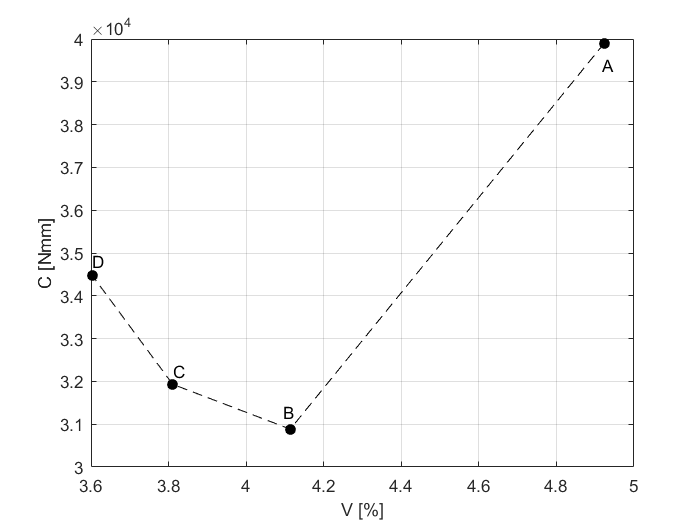
\includegraphics[width=0.5\textwidth]{images/Ch2/pareto2}
       }
       \caption{Pareto front obtained varying the allowable aggregated TSFC variation ($T_0$) in equation  \ref{topoeq3}.  . a) $V$ vs $\Delta TSFC$ \% corresponding to each solution. b) $V$ vs $C$ \% corresponding to each solution.   }
       \label{fig.B21}
\end{figure}
\begin{figure}[ht]
 \centering
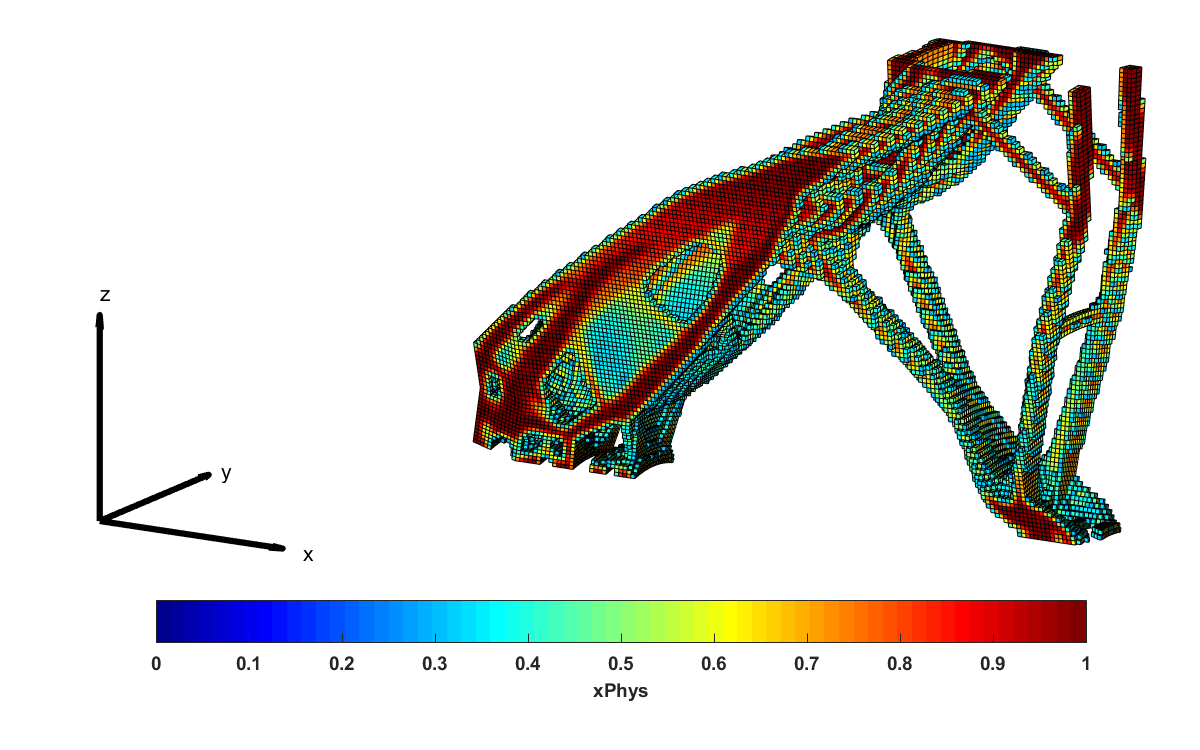
\includegraphics[width=\textwidth]{images/Ch2/SOL_A}
 \caption{Density plot of solution A obtained with $T_0=0.16$}
\label{fig.B22}
\end{figure}
\begin{figure}[ht]
 \centering
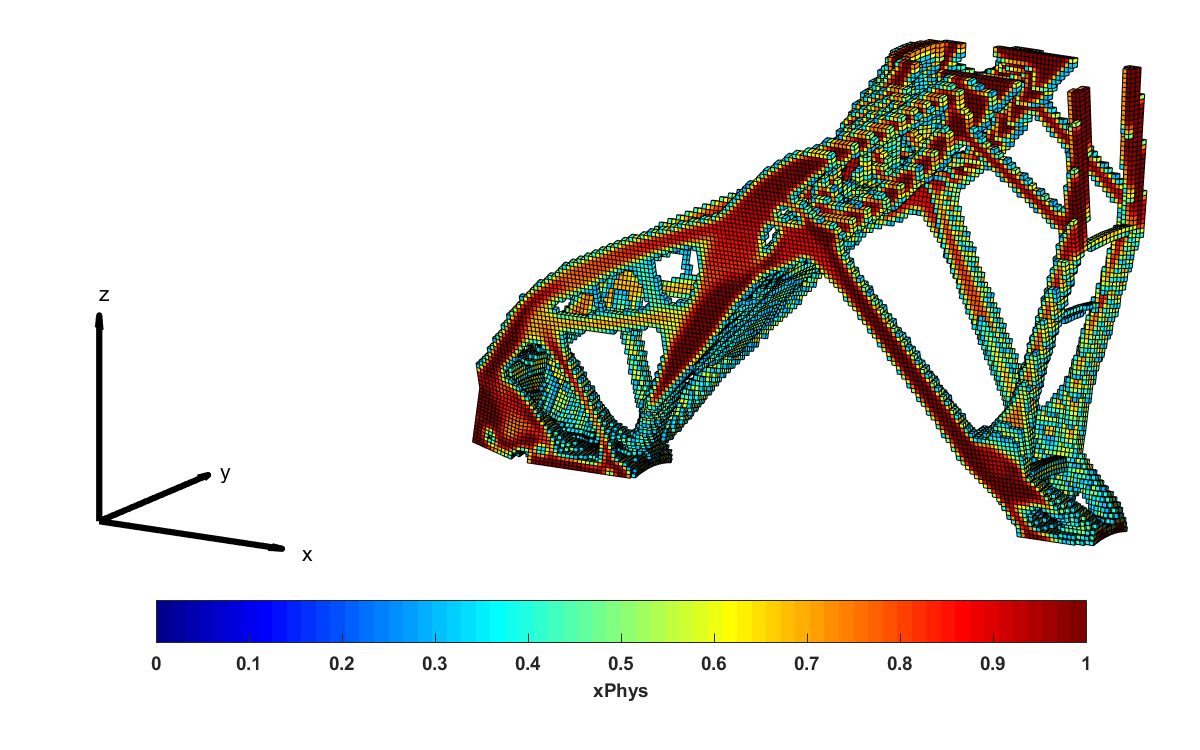
\includegraphics[width=\textwidth]{images/Ch2/SOL_B}
 \caption{Density plot of solution B obtained with $T_0=0.17$}
\label{fig.B23}
\end{figure}
\begin{figure}[ht]
 \centering
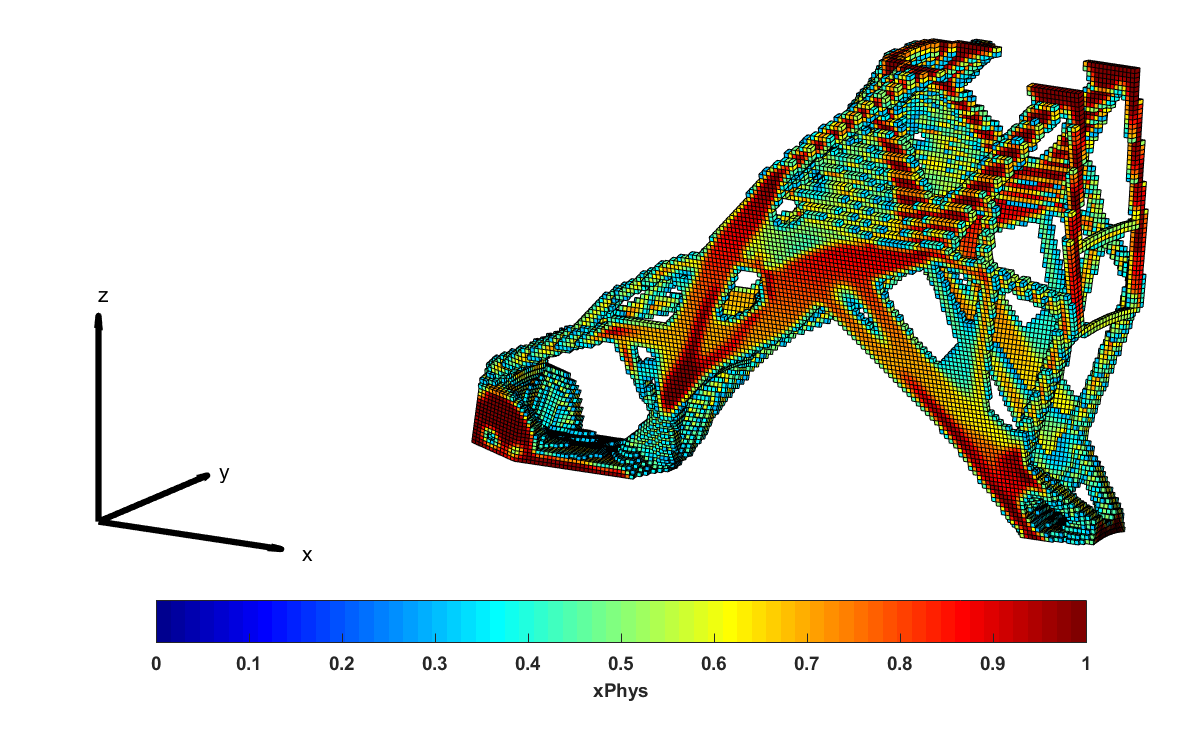
\includegraphics[width=\textwidth]{images/Ch2/SOL_C}
 \caption{Density plot of solution C obtained with $T_0=0.18$}
\label{fig.B24}
\end{figure}
\begin{figure}[ht]
 \centering
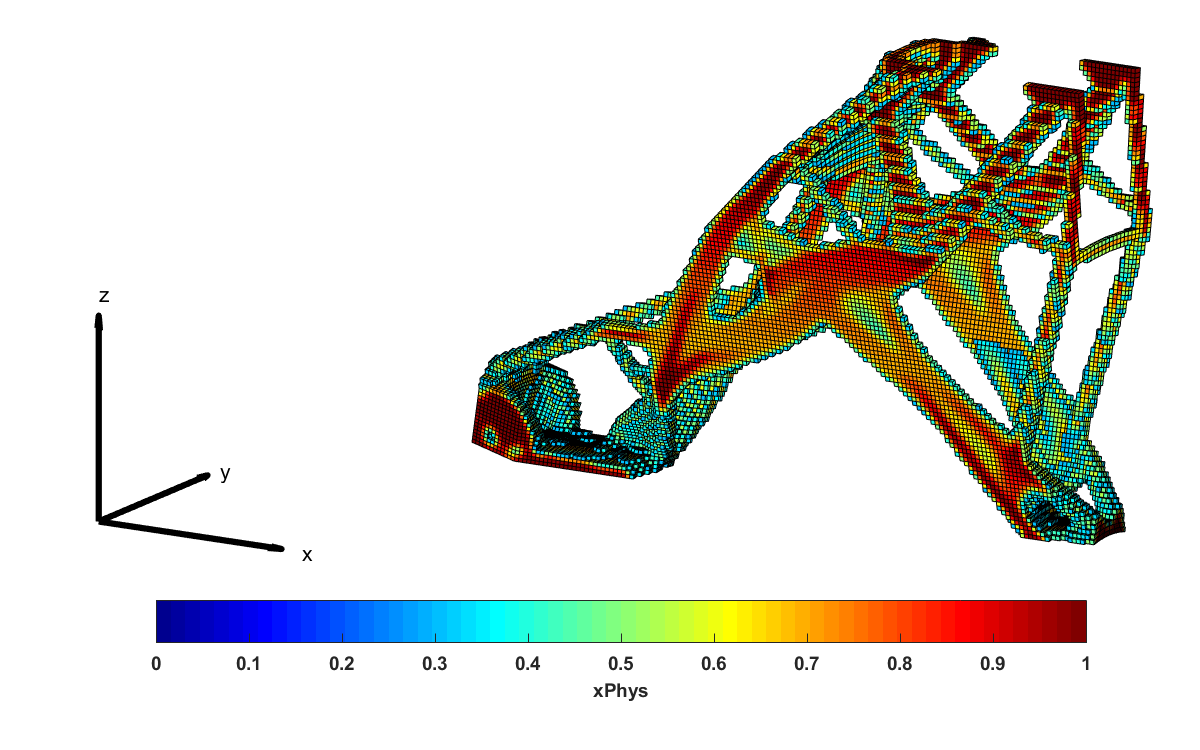
\includegraphics[width=\textwidth]{images/Ch2/SOL_D}
 \caption{Density plot of solution D obtained with $T_0=1$}
\label{fig.B25}
\end{figure}